\chapter{Dostępne systemy monitorujące}
\label{chap:Systemy}

\section[Przegląd systemów][Przegląd systemów dostępnych na rynku]{Przegląd systemów dostępnych na rynku}

Na rynku dostępnych jest wiele bardzo różnych systemów
monitorujących. Narzędzia z~tej grupy możemy podzielić na dwie
kategorie:

\begin{itemize}
\item Systemy dostępnościowe,
\item Systemu analityczne.
\end{itemize}

Systemy monitorujące w~których główny nacisk położony jest na
zapewnienie ciągłej dostępności monitorowanych usług nazywane są
systemami dostępnościowymi. Wspierają one administratora
w~codziennych zadaniach, poprzez nieustanne monitorowanie aktualnego
stanu sieci. Narzędzia te są wykorzystywane przede wszystkim do
szybkiego powiadamiania oraz lokalizacji awarii.

Systemy analityczne, w~kontekście monitorowania infrastruktury
sieciowej, to systemy, które są nastawione na zbieranie i~analizę
posiadanych danych. Tego typu systemy nie są zazwyczaj wykorzystywane
do powiadamiania czy lokalizacji awarii. Ich zadaniem jest przede
wszystkim gromadzenie danych dotyczących zużycia poszczególnych
zasobów, czy też wskaźników jakości poszczególnych usług. Systemy te
posiadają zazwyczaj bardzo rozbudowane narzędzia służące do generacji
i~analizy wykresów na podstawie zebranych wcześniej danych.

W~ostatnich latach można zauważyć wzrost popularności rozwiązań
hybrydowych. Pozwalają one na kompleksowe zarządzanie infrastrukturą
sieciową. Dzięki zastosowaniu takiego systemu administrator uzyskuje
jeden uniwersalny interfejs. Możliwy jest w nim zarówno pogląd
bieżącego stan sieci oraz diagnoza awarii, jak i~analiza danych
historycznych.

Przechowywanie danych zgromadzonych podczas monitorowania może odbywać
się na różne sposoby. Podstawową techniką przechowywania danych,
jeszcze 5 lat temu były płaskie struktury pliki zawierające
zgromadzone dane. Rozwiązanie tego typu jest bardzo uciążliwe,
a~sprawne zarządzanie zgromadzonymi danymi wymaga dużego wkładu pracy
własnej administratora. Obecnie rozpowszechniają się techniki
przechowywania zebranych danych w~oparciu o~bazy danych. Współcześnie
używane typy baz danych to:

\begin{itemize}
\item Relacyjne bazy danych
\item Cykliczne bazy danych\footnote{ang. {\em Round Robin Database}}
\end{itemize}

Dane przechowywane w~relacyjnych bazach danych zorganizowane są
w~postaci tabel, a~powiązania pomiędzy danymi nazywane są
relacjami. Taka organizacja bazy danych sprawia, że wraz z~upływem
czasu jej rozmiar rośnie. Powoduje to zwiększenie zajętości
przestrzeni dyskowej, a~także wpływa na czas wykonywania
operacji. Dane są przechowywane w~bazie do czasu, gdy użytkownik
jawnie je usunie. Pozwala to na przeglądanie dowolnie długiego okresu
historii, bez utraty dokładności, a~także na dynamiczne zarządzanie
czasem przechowywania danych. Narzędzia korzystające z~tego typu baz
muszą posiadać pewną politykę zarządzania zgromadzonymi danymi. Istotne
jest jednak, że polityka ta jest uzależniona jedynie od aplikacji,
a~nie od samej bazy danych i~może być zmieniana w dowolnym momencie.

Cykliczne bazy danych posiadają natomiast stały, definiowany podczas
tworzenia rozmiar. Rozmiar ten określa liczbę porcji danych jaka może
być przechowywana w~bazie. Jeśli rozmiar bazy przekroczy rozmiar
zadany przy tworzeniu, wykonywana jest konsolidacja danych. Polega ona
na wyliczeniu zadanych wartości w~odpowiednich przedziałach
i~zachowanie ich w~pojedynczych rekordach, oraz usunięcie dokładnych
danych. Możliwe są trzy typy konsolidacji danych, minimum, średnia
oraz maksimum. Rozmiar bazy danych jest definiowany w~chwili jej
tworzenia i~późniejsza jego modyfikacja nie jest już możliwa. Ponadto
należy zwrócić szczególną uwagę, na fakt iż dane są usuwane z~bazy
danych bez wiedzy użytkownika czy aplikacji, przez co taka baza danych
nie może zostać użyta do dokładnej analizy danych historycznych.

Każdy typ systemu, jak i~rodzaj bazy danych posiada swoje
zastosowanie. Należy zatem rozważnie zdefiniować wymagania jakie
stawia się przed systemem. Precyzyjne sformułowanie wymagań oraz
dokładna analiza możliwości każdego z~systemów zapewni wybór narzędzia
dostosowanego do potrzeb. Możliwa jest jednak sytuacja, w~której żaden
z~dostępnych systemów, nie będzie spełniał wszystkich stawianych
wymagań. Konieczne jest w~takiej sytuacji podjęcie wysiłku modyfikacji
systemu spełniającego najwięcej wymagań, lub zaprojektowanie oraz
implementacja takiego systemu od podstaw.

\subsection[Cacti][System monitorowania Cacti]{System monitorowania Cacti}

Jest to system monitorujący, rozwijany przez The Cacti Group
Inc. i~dystrybuowany na licencji~GPL\footnote{ ang. {\em General
    Public License} - popularna licencja oprogramowania o~otwartych
  źródłach. Treść licencji można znaleźć w~\cite{www:GPLv2}.}. System
bazuje na oprogramowaniu RRDtool. Jest to narzędzie, które pozwala na
wykorzystanie cyklicznej bazy danych do składowania pomiarów wartości
w zadanym przedziale czasowym. Ponadto dostarcza ono funkcji do
generacji wykresów w~kilku formatach. Dokładny opis wszystkich
możliwości RRDTool można znaleźć w~\cite{www:RRDtool}. Dzięki
wykorzystaniu wspomnianego narzędzia system ma bardzo prostą budowę
i~składa się z~następujących elementów:

\begin{itemize}
\item interfejs użytkownika,
\item dostawca danych.
\end{itemize}

Interfejs użytkownika został napisany w~języku PHP. Do jego działania
niezbędny jest serwer http np. Apache. Rysunek
\ref{fig:CactiInterface} przedstawia przykładową podstronę systemu
Cacti. Z~poziomu interfejsu użytkownika możliwa jest graficzna
konfiguracja całego systemu. Interfejs posiada klasyczna
budowę. Składa się on z~jednokolorowego paska menu, w~którym zawarte
są odnośniki do poszczególnych podstron oraz z~pulpitu, na którym
wyświetlane są wybrane dane. Interfejs umożliwia graficzne
przedstawienie wyników w~postaci wykresów. Format wykresu może być
definiowany bezpośrednio przez użytkownika, lub można skorzystać
z~bogatej biblioteki gotowych szablonów. Dostęp do interfejsu
zabezpieczony jest poprzez mechanizm uwierzytelnienia użytkownika
systemu monitorującego. Możliwe jest definiowanie wielu użytkowników
oraz ich uprawnienia. Każdy użytkownik ma możliwość definiowania
własnego zestawu wykresów oraz pulpitów.

%czy trzeba dawać to do źródel?
\begin{figure}[h]
\label{fig:CactiInterface}
\caption{Interfejs użytkownika systemu Cacti.}
\begin{center}
\makebox[\textwidth]{%
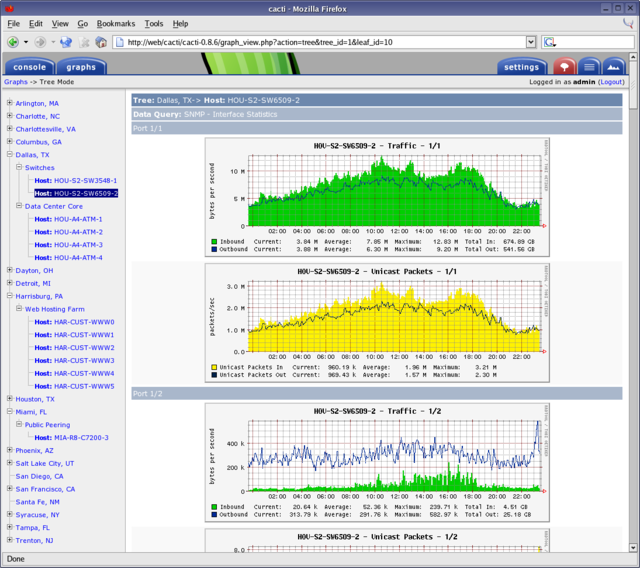
\includegraphics[width=1\textwidth]{img/cacti.png}
}\\[0.1cm]
\end{center}
\end{figure}


Dostawca danych jest to element systemu, który jest odpowiedzialny za
faktyczne wykonywanie sprawdzeń danej wartości i~przekazywanie ich do
narzędzia RRDTool. System umożliwia wybór jednego z~dwóch dostawców
danych. Pierwszym z~nich jest cmd.php, który jest prostym skryptem
napisanym w języku PHP. Umożliwia on monitorowanie aktywne urządzeń
przy pomocy protokołu SNMP\footnote{ {\em Simple Network Management
    Protocol} -- protokół zarządzania urządzeniami sieciowymi
  i~uzyskiwania informacji o~ich stanie. Zorganizowany w~formie
  drzewa, gdzie każdy liść posiada globalnie unikalny identyfikator
  o~ściśle określonym znaczeniu. Szeroko opisany w \cite{www:SNMP}.}. Skrypt
cmd.php przeznaczony jest do monitorowania jedynie niewielkich
sieci. Ze względów wydajnościowych, nie jest możliwe wykorzystanie go
do monitorowania rozległej infrastruktury.

Drugim z~możliwych do wyboru dostawców danych jest narzędzie Spine,
nazywany również Cactid. Jest to program napisany w~języku~C, który
uruchomiony jest jako serwis systemowy na urządzeniu
monitorującym. Umożliwia on monitorowanie urządzeń zarówno poprzez
protokół SNMP jak i~z~wykorzystaniem innych metod. Możliwość
dostarczenia własnych metod monitorowania opiera się na dostarczeniu
skryptu lub pliku wykonywalnego, który będzie cyklicznie uruchamiany
przez Cactid, a~jako wyniki przekazywane w taki sam sposób jak
z~sprawdzeń opierających się na SNMP.

Żaden z~dostawców danych nie umożliwia monitorowania danego urządzenia
lub usługi w~sposób pasywny. Cacti nie posiada również żadnego
mechanizmu, który pozwoliłby na monitorowanie sieci w~sposób
rozproszony. Oznacza to, iż administrator musi zmienić konfigurację
sieci, tak aby jeden serwer miał dostęp do każdego urządzenia, lub
konfigurować i~zarządzać osobną instancją w~każdym segmencie. Jest to
bardzo niewygodne i~wręcz uniemożliwia monitorowania rozległych sieci
przy pomocy Cacti\footnote{Więcej informacji na temat systemu
  monitorowania Cacti można znaleźć w~\cite{www:Cacti}.}.

\subsection[Nagios][System monitorowania Nagios]{System monitorowania Nagios}

System Nagios został opublikowany w~1999 na licencji GPL. System od
niemal 15 lat jest ciągle rozwijany i~udoskonalany, zarówno przez
autorów jak i~przez szeroką społeczność. W~systemie Nagios najwyższym
priorytetem jest dbałość o~zapewnienie dostępności wszystkich
monitorowanych usług. Organizacja systemu zakłada, iż w~sieci znajdują
się urządzenia, które mogą świadczyć pewne usługi. Każde urządzenie
jak i~usługa może być w jednym z trzech stanów logicznych:

\begin{description}
\item[OK] usługa działa poprawnie
\item[WARNING] monitorowane parametry przekroczyły stan ostrzegawczy
\item[CRITICAL] parametry usługi przekroczyły stan krytyczny, usługa
  lub urządzenie nie funkcjonuje
\end{description}

System posiada rozbudowane algorytmy określania stanu każdego
urządzenia oraz usługi. Działanie usługi, jest zawsze zależne od stanu
urządzenie, na którym dana usługa jest świadczona. Ponadto użytkownik
może definiować zależności pomiędzy urządzeniami. System Nagios
posiada rozbudowany system powiadamiania administratora o~wystąpieniu
awarii oraz o~jej zakończeniu, lub innych zdefiniowanych wydarzeniach
systemowych. Ponadto możliwe jest automatyczne wykonywanie programów
lub skryptów, jeśli wystąpiło jakieś zdarzenie. Podstawowa wersja
systemu składa się z następujących elementów:

\begin{itemize}
\item Interfejs graficzny
\item Rdzeń monitorujący
\end{itemize}

Interfejs graficzny został napisany w~języku~C z~wykorzystaniem
technologi CGI\footnote{{\em Common Gateway Interface} --
  znormalizowany interfejs służący do komunikacji pomiędzy serwerem
  www, a~zewnętrznymi programami. Interfejs ten jest wykorzystywany do
  generowania stron internetowych na żądanie klienta. Zewnętrzny
  program generuje stronę w~języku HTML, a~następnie serwer przesyła
  ją do klienta poprzez serwer http. Szczegółowy opis można znaleźć
  w~\cite{www:CGI}}. Jego wygląd jest zgodny z~standardami z~lat
90. Klasyczna strona WWW bez dynamicznie zmieniającej się treści. Dane
odświeżane są na żądanie klienta, lub co określony czas. Wykorzystana
technologia zakłada przesyłanie za każdym razem całego dokumentu HTML
do klienta, w~związku z~czym generowany jest nadmierny ruch
sieciowy. Widok użytkownika składa się z~kliku części. Po lewej
stronie widoczne jest klasyczne menu, umożliwiające użytkownikowi
wybór treści. Na górze strony natomiast znajduje się podsumowanie
aktualnego stanu monitorowanych urządzeń i~usług. Centralną część okna
zajmuje pulpit, który prezentuje użytkownikowi treść wybraną wcześniej
z~menu. Interfejs użytkownika umożliwia podgląd aktualnego stanu usług
oraz urządzeń. Informacja ta może być wyświetlana w~formie listy
zawierającej urządzenia i~usługi, lub w~postaci mapy sieci, która
pozwala na monitorowanie stanu urządzenia w~korelacji z~jego logicznym
umieszczeniem w~strukturze sieciowej. Możliwe jest również
przeglądanie historii awarii oraz prostych wykresów stanu urządzenia
lub usługi w~zadanym przedziale czasu. Dostęp do interfejsu chroniony
jest przy pomocy autoryzacji http. Możliwe jest definiowanie wielu
użytkowników, jednak tylko z~poziomu urządzenia na którym uruchomiony
jest system monitorujący. Należy zauważyć również, że wszyscy
użytkownicy danego typu posiadają takie same uprawnienia. Nie ma
możliwości dowolnej edycji uprawnień danej grupy czy też użytkownika.

%czy prawa autorskie?
\begin{figure}[h]
\label{fig:NagiosInterface}
\caption{Interfejs użytkownika systemu Nagios.}
\begin{center}
\makebox[\textwidth]{%
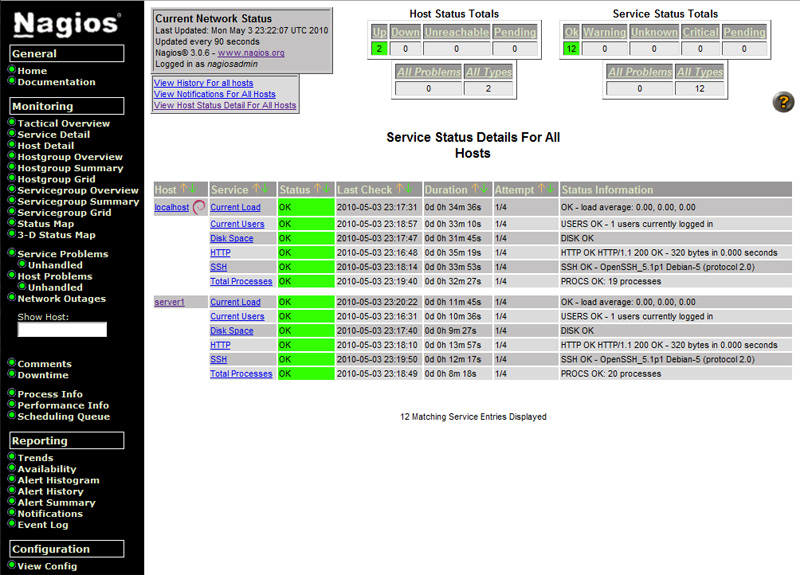
\includegraphics[width=1\textwidth]{img/nagios.jpg}
}\\[0.1cm]
\end{center}
\end{figure}

Rdzeń monitorujący został zaimplementowany w~języku C. Jest to centrum
całego systemu, gdyż zajmuje się on przetwarzaniem wszystkich
bieżących danych monitorowania, a~następnie składowaniem ich
w~plikach. Ta cześć systemu jest odpowiedzialna za wykonywanie
sprawdzeń w~określonych odstępach czasu. Każde sprawdzenie odbywa się
poprzez wykonanie komendy zdefiniowanej przez użytkownika. Komenda ta
może zawierać zarówno wykonanie pliku binarnego jak i~dowolnego
skryptu. W~ramach projektu Nagios, rozwijany jest zestaw
wtyczek\footnote{Należy zwrócić uwagę na różne znaczenie słów wtyczka
  (ang. {\em Plugin}) oraz dodatek (ang. {\em Addon}). }, czyli
programów służących do monitorowania podstawowych usług oraz
parametrów urządzeń. Dostępna jest bardzo duża liczba wtyczek, dzięki
czemu system Nagios może monitorować w~sposób aktywny wszystkie
podstawowe parametry lub usługi. Możliwe jest również definiowanie
własnych wtyczek, które będą sprawdzały stany pewnych specyficznych
dla danej sieci parametrów. W~celu zapewnienia poprawnego
funkcjonowania całego systemu, konieczne jest, aby dodatkowe wtyczki
spełniały wymagania opisane w~\cite{www:NagiosPluginsTutorial}. System
umożliwia również monitorowanie dowolnych usług w~sposób
pasywny. Programy dostarczające odczytów pasywnych również są
zobowiązane do przestrzegania wcześniej wspomnianych zasad.

System posiada rozbudowane możliwości monitorowania
rozproszonego. Niestety, do wykonania znacznej części z~tych
konfiguracji potrzebne są elementy systemu, które są dystrybuowane na
licencjach komercyjnych wymagających zakupu praw do korzystania z
nich. Istnieją również darmowe dodatki, które pozwalają na
przechowywanie zgromadzonych danych zarówno w~bazie relacyjnej jak
i~cyklicznej. Możliwa jest również częściowa integracja systemu
Nagios\footnote{Szczegółowe informacje na temat rozszerzania
  funkcjonalności oraz samego systemu można znaleźć
  w~\cite{www:Nagios}.}  z~dodatkami lub systemami, które pozwalają na
wizualizacje zgromadzonych danych.

\subsection[Icinga][System monitorowania Icinga]{System monitorowania Icinga}
\label{subsec:Icinga}

System Icinga powstał w~2009 roku jako klon (ang. {\em fork}) systemu
Nagios. System został wzbogacony o~wiele nowych elementów, a~także
poprawiono wiele błędów obecnych w~systemie Nagios. Dzięki zachowaniu
wstecznej kompatybilności zarówno wszystkie wtyczki jak i~dodatki
systemu Nagios mogą być wykorzystane w~systemie Icinga. Pozyskano
dzięki temu bardzo dużą bazę wtyczek, co umożliwia monitorowanie tych
samych usług i~urządzeń co przodek.

System Icinga został wyposażony w~zupełnie nowy interfejs
graficzny\footnote{Skorzystanie z nowego interfejsu wymaga użycia
  modułu IDOUtils oraz bazy danych. Możliwe jest wykorzystanie również
  klasycznego interfejsu, który nie posiada takich wymagań.}. Został
on zaimplementowany w~języku PHP przy użyciu szkieletu aplikacji
agavi\footnote{{\em Agavi } -- szkielet aplikacji języka PHP5
  pozwalający na łatwą realizację funkcjonalności zgodne z~modelem
  programowym Model-Widok-Kontroler. Szerszy opis znajduje się na
  stronie domowej projektu: \cite{www:Agavi}}. Jest on zatem oparty na
technologii Ajax, dzięki której komunikacja z~użytkownikiem, nie opiera
się na przesyłaniu całych stron w~języku HTML, lecz na realizacji
żądań generowanych poprzez język skryptowy wykonywany po stronie
użytkownika. Dzięki zastosowaniu tej technologi, proces wyświetlania
strony zużywa mniejszą część pasma, a~serwer został odciążony. Nowy
interfejs użytkownika jest w~pełni dynamiczny, składa się on
z~rozszerzalnego menu po lewej stronie oraz pulpitów użytkownika
w~centralnej części. Możliwe jest otwieranie wielu pulpitów oraz
wyświetlanie poszczególnych informacji w~osobnych oknach, które można
swobodnie przemieszczać w~obszarze strony. Przykładowy pulpit dostępny
dla użytkownika został przedstawiony na
\ref{fig:IcingaInterface}.Znacznej zmianie uległ również model
bezpieczeństwa. W~nowym interfejsie graficznym, każdy użytkownik,
posiada swój zestaw zdefiniowanych uprawnień. Oznacza to, że możliwe
jest ograniczenie użytkownikowi dostępu do danych o~konkretnej usłudze
lub zabronić wykonywania niektórych czynności
administracyjnych. Zarządzanie użytkownikami oraz ich uprawnieniami
możliwe jest również z~poziomu graficznego interfejsu użytkownika, co
znacząco podnosi wygodę użytkowania systemu.

\begin{figure}[h]
\label{fig:NagiosInterface}
\caption{Interfejs użytkownika systemu Icinga.}
\begin{center}
\makebox[\textwidth]{%
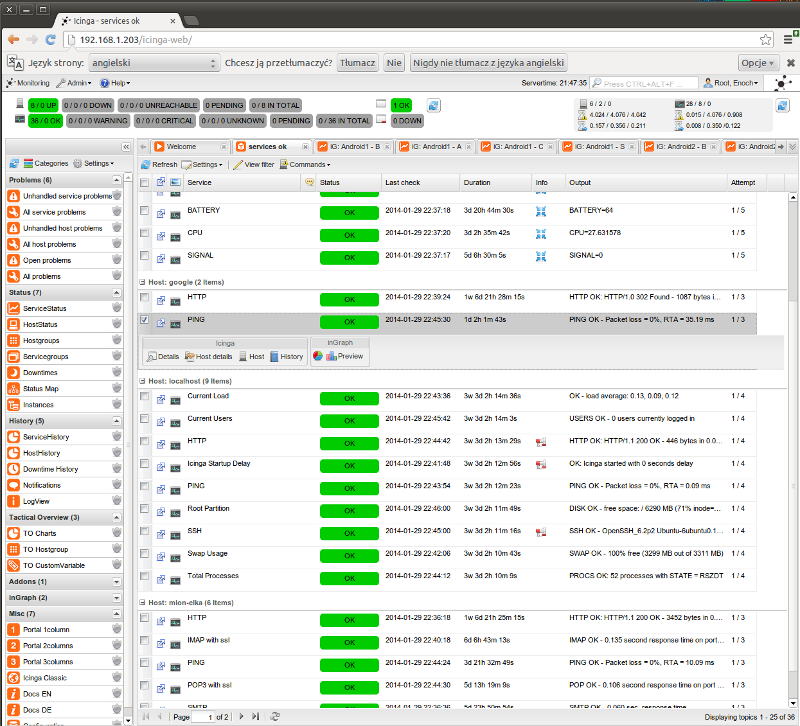
\includegraphics[width=1\textwidth]{img/icinga.png}
}\\[0.1cm]
\end{center}
\end{figure}

Kolejną istotną różnicą, jest zmiana architektury systemu. System
Nagios posiada budowę monolityczną, a~współpraca pomiędzy
poszczególnymi jego komponentami odbywa się w~sposób bardzo zawiły
i~niejednorodny. System Icinga wprowadził natomiast budowę
modularną. Wszystkie możliwe komponenty systemu zostały wyodrębnione,
a~do swobodnej komunikacji pomiędzy nimi zdefiniowano wygodne
API. Taka budowa umożliwia przede wszystkim rozmieszczenie
poszczególnych komponentów systemu na różnych fizycznych maszynach, co
w~przypadku dużych sieci może spowodować znaczący wzrost wydajności
i~niezawodności. Dostarczenie jednolitego REST API\footnote{ang. {\em
    Representational state transfer} -- lekka metoda przesyłania
  danych pomiędzy klientem a~serwerem.} umożliwia również prostsze
tworzenie dodatków rozbudowujących możliwości systemu.  W~systemie
Icinga rozbudowano także możliwości współpracy z~bazą danych. System
ten umożliwia współpracę, już nie tylko z~bazą MySQL, lecz również
z~bazami PostgreSQL czy też z~systemem zarządzania bazą danych firmy
Oracle. Możliwość wykorzystania bazy danych Oracle, jest bardzo
istotna, jeśli dane dotyczące konfiguracji muszą być przechowywane
przez bardzo długi czas, lub jeśli monitorowana infrastruktura jest
bardzo rozbudowana.

System Icinga, nie tylko umożliwia rozmieszczenie modułów na różnych
fizycznych maszynach, lecz również umożliwia wiele innych
konfiguracji, które można wykorzystać podczas monitorowania
rozproszonego. Szczególnie wartą zauważenia jest konfiguracja,
w~której występuje wiele równorzędnych instancji rdzenia
monitorującego, natomiast wszystkie współpracują używając jednej bazy
danych. Centralna baza danych stanowi źródło danych dla interfejsu
graficznego. Taka konfiguracja umożliwia monitorowanie bardzo
rozległej lub wielosegmentowej infrastruktury i prezentacji wyników
poprzez jeden interfejs. Należy również nadmienić, iż wszystkie
elementy niezbędne do konfiguracji takiego rozwiązania są darmowe.

\section[Podsumowanie][Podsumowanie]{Podsumowanie}

Współczesne systemy monitoringu, są bardzo bogato wyposażone
i~posiadają szereg zaawansowanych możliwości. Każdy z~systemów oferuje
unikalny zestaw rozwiązań, które z~pewnością mogą zostać wykorzystane
w~wielu instytucjach. Porównując wszystkie omówione systemy, należy
zwrócić szczególną uwagę, na różnice w~ich możliwych zastosowaniach
docelowych.

Systemy, takie jak Cacti zaliczane są do grupy systemów
analitycznych. Ich celem jest zatem zapewnienie możliwości gromadzenia
oraz analizy danych. Zbierane dane mają charakter zagregowany
w~zadanych przedziałach, na podstawie których prezentowane są
użytkownikowi odpowiednie wykresy. Niestety ze względu na główny
sposób gromadzenia danych - protokół SNMP, oraz ubogość innych metod,
systemy te nie mogą być wzbogacone o~funkcjonalność charakterystyczną
dla systemów dostępnościowych.

Drugą grupę systemów stanowią natomiast systemy dostępnościowe, takie
jak Nagios czy Icinga. Ich głównym celem jest monitorowanie bieżącego
stanu infrastruktury i~raportowanie użytkownikowi najświeższych
informacji. Systemy te zostały również zaprojektowane, aby wspomagać
administratora w~lokalizacji awarii. Głównym typem danych na których
operują te systemy jest stan urządzenia lub usługi. Zdefiniowanie
odpowiednich poziomów kwantyzacji dla stanów pozwala na szybkie
uzyskiwanie poglądowych informacji o~stanie sieci. Podczas
monitorowania gromadzone są również dane szczegółowe. Ich
przetwarzaniem nie zajmują się już jednak same systemy monitorowania,
lecz liczne dodatki do nich. Możliwe jest zatem rozbudowanie systemu
tego typu, o~dodatkowe elementy, które pozwolą uzyskać system
hybrydowy. System taki będzie mógł pełnić rolę zarówno systemu
dostepnościowego jak i analitycznego.

Wybierając system monitorujący, należy zatem dokonać szczegółowej
analizy wymagań stawianych przed systemem. Szczegółowe porównanie
wszystkich przedstawionych systemów monitorowania zawarto
w~\ref{tab:PorownanieSys}.

\begin{longtable}[c]{|p{4.5cm}||p{3cm}|p{3cm}|p{3cm}|}
  \caption[Porównanie systemów monitorowania]{Porównanie systemów monitorowania} \label{tab:PorownanieSys} \\
  \hline \multicolumn{1}{|c||}{Nazwa systemu} &
  \multicolumn{1}{c|}{Cacti} & \multicolumn{1}{c|}{Nagios} &
  \multicolumn{1}{c|}{Icinga} \tabularnewline \hline \hline
  \endfirsthead

  \multicolumn{4}{c}%
  {{\tablename\ \thetable{} -- Kontynuacja z~poprzedniej strony}} \\
  \hline
  \multicolumn{1}{|c||}{Nazwa systemu} &
  \multicolumn{1}{c|}{Cacti} & \multicolumn{1}{c|}{Nagios} &
  \multicolumn{1}{c|}{Icinga} \tabularnewline 
  \hline \hline
  \endhead

  \hline \multicolumn{4}{|r|}{{Kontynuacja na następnej stronie}} \\ \hline
  \endfoot

  \hline\hline
  \endlastfoot

  \raggedright{Podgląd stanu bieżącego} & \raggedright{Nie} &
  \raggedright{Ta}k & \raggedright{Ta}k \tabularnewline 
  \hline

  \raggedright{Podgląd danych historycznych} &\raggedright{Tak} &
  \raggedright{Tak, przez dodatek} & \raggedright{Tak, przez dodatek}
  \tabularnewline
  \hline

  \raggedright{Dane w~formie wykresu} & \raggedright{Tak} &
  \raggedright{Tak, przez dodatek} & \raggedright{Tak, przez dodatek}
  \tabularnewline 
  \hline

  \raggedright{Przechowywanie danych w~bazie cyklicznej} & \raggedright{Tak} &
  \raggedright{Tak, przez dodatek} & \raggedright{Tak, przez dodatek}
  \tabularnewline
  \hline

  \raggedright{Przechowywanie danych w~bazie relacyjnej} & \raggedright{Nie} &
  \raggedright{Tak, przez dodatek} & \raggedright{Tak, przez dodatek}
  \tabularnewline
  \hline

  \raggedright{Powiadomienia o~awarii} & \raggedright{Nie} &
  \raggedright{Tak, email lub telefon} & \raggedright{Tak, email lub telefon}
  \tabularnewline
  \hline

  \raggedright{Wsparcie w~lokalizacji awarii} & \raggedright{Nie} &
  \raggedright{Tak, poprzez mapę logiczną sieci} & \raggedright{Tak, poprzez mapę logiczną sieci}
  \tabularnewline
  \hline

  \raggedright{Obsługa SNMP} & \raggedright{Tak} &
  \raggedright{Tak, przez wtyczkę} & \raggedright{Tak, przez wtyczkę}
  \tabularnewline
  \hline

  \raggedright{Zbieranie danych spoza SNMP} & \raggedright{Tak, niewielka liczba dostępnych metod} &
  \raggedright{Tak, bogaty zestaw wtyczek} & \raggedright{Tak, bogaty zestaw wtyczek}
  \tabularnewline
  \hline

  \raggedright{Monitorowanie pasywne} & \raggedright{Nie} &
  \raggedright{Tak} & \raggedright{Tak}
  \tabularnewline
  \hline

  \raggedright{Nowoczesny interfejs użytkownika} & \raggedright{Nie} &
  \raggedright{Nie} & \raggedright{Tak, z wykorzystaniem technologi AJAX}
  \tabularnewline
  \hline

  \raggedright{Wielu użytkowników} & \raggedright{Tak} &
  \raggedright{Tak} & \raggedright{Tak}
  \tabularnewline
  \hline

  \raggedright{Metoda uwierzytelnienia} & \raggedright{Uwierzytelnienie wewnętrzne} &
  \raggedright{Uwierzytelnienie http} & \raggedright{Uwierzytelnienie wewnętrzne}
  \tabularnewline
  \hline

  \raggedright{Zarządzanie kontami użytkowników z~interfejsu} & \raggedright{Tak} &
  \raggedright{Nie} & \raggedright{Tak}
  \tabularnewline
  \hline

  \raggedright{Definiowanie uprawnień dla użytkowników} & \raggedright{Tak, przez interfejs graficzny} &
  \raggedright{Nie} & \raggedright{Tak, przez interfejs graficzny}
  \tabularnewline
  \hline

  \raggedright{Molarność} & \raggedright{Nie} &
  \raggedright{Nie} & \raggedright{Tak}
  \tabularnewline
  \hline

  \raggedright{Rozmieszczenie modułów na różnych urządzeniach fizycznych} & \raggedright{Nie dotyczy} &
  \raggedright{Nie dotyczy} & \raggedright{Tak}
  \tabularnewline
  \hline

  \raggedright{Możliwość monitorowania rozproszonego z~instancją
    nadrzędną} & \raggedright{Nie} & \raggedright{Tak} &
  \raggedright{Tak}
  \tabularnewline
  \hline

  \raggedright{Możliwość monitorowania rozproszonego bez instancji nadrzędnej} & \raggedright{Nie} &
  \raggedright{Tak, konieczny płatny dodatek} & \raggedright{Tak}
  \tabularnewline
  \hline

  \raggedright{Generacja raportów} & \raggedright{Nie} &
  \raggedright{Nie} & \raggedright{Tak, z~wykorzystaniem JasperReports}
  \tabularnewline
  \hline

  \raggedright{Możliwość monitorowania klienta mobilnego} & \raggedright{Nie} &
  \raggedright{Nie} & \raggedright{Nie}
  \tabularnewline
  \hline

  \raggedright{Dostępność} & \raggedright{Darmowy} &
  \raggedright{Częściowo darmowy, wiele płatnych elementów i~funkcjonalności} & \raggedright{Darmowy}
  \tabularnewline
  \hline

  \raggedright{Licencja} & \raggedright{GPL v2} &
  \raggedright{GPL v3 (tylko darmowe elementy)} & \raggedright{GPL v2}
  \tabularnewline
  \hline

\end{longtable}

Przedstawione systemy monitorujące w~znacznym stopniu zaspokajają
zapotrzebowanie rynku na systemy monitorowania. Pojawia się jednak
pewna nisza związana z~monitorowaniem urządzeń mobilnych. Zadanie to
nie jest trywialne i~wymaga obecności dodatkowych mechanizmów zarówno
na urządzeniu mobilnym, jak i~w~innych elementach systemu. Żaden
z~analizowanych systemów nie posiadał w~swej implementacji ani
w~oficjalnych repozytoriach z~dodatkami, oprogramowania, które
pozwalałoby na monitorowanie parametrów urządzenia mobilnego.

